%!TEX root = ../../book_ML.tex
\chapter{Hồi quy tuyến tính}
\label{cha:linear_regression}
\index{hồi quy tuyến tính -- linear regression}
% Trong chương này, chúng ta cùng làm quen với một trong những thuật toán machine
% learning  cơ bản nhất -- linear regression (hồi quy tuyến tính). Qua chương này,
% bạn đọc sẽ có cái nhìn ban đầu về việc xây dựng một hệ thống machine learning.
% Linear regression là một thuật toán supervised, ở đó quan hệ giữa đầu vào và đầu
% ra được mô tả bởi một hàm tuyến tính. Thuật toán này còn được gọi là
% \textit{linear fitting} hoặc \textit{linear least square}.

\textit{Hồi quy tuyến tính} (linear regression) là một thuật toán hồi quy mà đầu ra là một hàm số tuyến tính của đầu vào. Đây là thuật toán đơn giản nhất trong nhóm các thuật toán học có giám sát. 
\section{Giới thiệu} 
Xét bài toán ước lượng giá của một căn nhà rộng $x_1 ~ \text{m}^2$, có $x_2$
phòng ngủ và cách trung tâm thành phố $x_3~ \text{km}$. Giả sử có một tập dữ liệu của 10000 căn nhà trong thành phố đó. Liệu rằng khi có một căn nhà
mới với các thông số về diện tích $x_1$, số phòng ngủ $x_2$ và khoảng cách tới
trung tâm $x_3$, chúng ta có thể dự đoán được giá $y$ của căn nhà đó không? Nếu
có thì hàm dự đoán $y = f(\bx)$ sẽ có dạng như thế nào. Ở đây, vector đặc
trưng $\bx = [x_1, x_2, x_3]^T$ là một vector cột chứa dữ liệu đầu vào,
đầu ra $y$ là một số thực dương.

% \textbf{Lưu ý về ký hiệu toán học:} \textit{trong các bài viết của tôi, các số
% vô hướng được biểu diễn bởi các chữ cái viết ở dạng không in đậm, có thể viết
% hoa, ví dụ $x_1, N, y, k$. Các vector được biểu diễn bằng các chữ cái thường
% in đậm, ví dụ $\mathbf{y}, \bx_1 $. Các ma trận được biểu diễn bởi các
% chữ viết hoa in đậm, ví dụ $\mathbf{X, Y, W} $.}
\index{vector trọng số -- weight vector}
Nhận thấy rằng giá nhà cao nến diện tích lớn, nhiều phòng ngủ và gần trung tâm thành phố. Từ đó, ta có thể mô hình đầu ra là một hàm đơn giản của đầu vào:
\begin{equation}
\label{eqn:3_1}
y \approx \hat{y} = f(\bx) = w_1 x_1 + w_2 x_2 + w_3 x_3 = \bx^T\bw,
\end{equation}
trong đó $\bw = [w_1, w_2, w_3]^T$ là \textit{vector trọng số} (weight vector) cần tìm. Mối quan hệ $y \approx f(\bx)$ như trong~\eqref{eqn:3_1} là một mối quan hệ tuyến tính.


% trong đó, $w_1, w_2, w_3$ là các hằng số,  $w_0$ còn được gọi là bias. 

Bài toán trên đây là bài toán dự đoán giá trị của đầu ra dựa trên vector đặc
trưng đầu vào. Ngoài ra, giá trị của đầu ra có thể nhận rất nhiều giá trị thực
dương khác nhau. Vì vậy, đây là một bài toán hồi quy. Mối quan hệ $\hat{y} =
\bx^T\bw$ là một mối quan hệ tuyến tính. Tên gọi \textit{hồi quy tuyến tính}
xuất phát từ đây.


% Bài toán chúng ta đang làm là một bài toán thuộc loại regression. Bài toán đi
% tìm các hệ số tối ưu $ \{w_1, w_2, w_3, w_0 \}$ chính vì vậy được gọi là bài
% toán Linear Regression.
\index{dau@đầu ra thực sự -- ground truth}
\index{dau@đầu ra dự đoán -- predicted output}
\index{sai số mô hình}
% \textbf{Chú ý:} 
% \begin{enumerate}

% Giá trị $y$ và $\hat{y}$ lần lượt được gọi là \textit{đầu ra thực sự} và \textit{đầu ra
% dự đoán} của mô hình. Nhìn chung, $y$ và $\hat{y}$ là hai giá trị khác nhau.
% Lượng khác nhau này còn được gọ là \textit{sai số mô hình}. Sai số càng nhỏ, mô
% hình càng tốt.

    % \item \textit{Linear} hay \textit{tuyến tính} hiểu một cách đơn giản
    % là \textit{thẳng, phẳng}. Trong không gian hai chiều, một hàm số được gọi là
    % \textit{tuyến tính} nếu đồ thị của nó có dạng một \textit{đường thẳng}.
    % Trong không gian ba chiều, một hàm số được goi là \textit{tuyến tính} nếu đồ
    % thị của nó có dạng một \textit{mặt phẳng}. Trong không gian nhiều hơn ba
    % chiều, khái niệm \textit{mặt phẳng} không còn phù hợp nữa, thay vào đó, một
    % khái niệm khác ra đời được gọi là \textit{siêu mặt phẳng}
    % (\textit{hyperplane}). Các hàm số tuyến tính là các hàm đơn giản nhất, vì
    % chúng thuận tiện trong việc hình dung và tính toán.

% \end{enumerate}

% Chúng ta sẽ được thấy trong các bài viết sau, \textit{tuyến tính} rất quan trọng
% và hữu ích trong các bài toán Machine Learning. Kinh nghiệm cá nhân tôi cho
% thấy, trước khi hiểu được các thuật toán \textit{phi tuyến} (non-linear, không
% phẳng), chúng ta cần nắm vững các kỹ thuật cho các mô hình \textit{tuyến tính}.

\section{Xây dựng và tối ưu hàm mất mát}

% \subsection{Dạng của Linear Regression }

% Trong phương trình \eqref{eqn:3_1} phía trên, nếu chúng ta đặt
% $\bw = [w_0, w_1, w_2, w_3]^T = $ là vector (cột) hệ số cần phải tối ưu
% và $\mathbf{\bar{x}} = [1, x_1, x_2, x_3]$ (đọc là \textit{x bar} trong tiếng
% Anh) là vector (hàng) dữ liệu đầu vào \textit{mở rộng}. Số $1$ ở đầu được thêm
% vào để phép tính đơn giản hơn và thuận tiện cho việc tính toán. Khi đó, phương
% trình (1) có thể được viết lại dưới dạng:

% \begin{equation}y \approx \mathbf{\bar{x}}\bw = \hat{y}\end{equation}

% Chú ý rằng $\mathbf{\bar{x}}$ là một vector hàng.

Tổng quát, nếu mỗi điểm dữ liệu được mô tả bởi một vector đặc trưng $d$ chiều $\bx \in \R^d$, hàm dự đoán đầu ra được viết dưới dạng
\begin{equation}
\label{eqn:3_10}
    y = w_1x_1 + w_2x_2 + \dots + w_dx_d = \bx^T\bw.
\end{equation}

\subsection{Sai số dự đoán}
Sau khi xây dựng được mô hình dự đoán đầu ra như~\eqref{eqn:3_10}, ta cần tìm
một phép đánh giá phù hợp với bài toán. Với bài toán hồi quy nói chung, ta
mong muốn sự sai khác $e$ giữa đầu ra thực sự $y$ và đầu ra dự đoán
$\hat{y}$ là nhỏ nhất:
\begin{equation}
    \frac{1}{2}e^2 = \frac{1}{2}(y - \hat{y})^2 =
    \frac{1}{2}(y - \bx^T\bw)^2.
\end{equation}
Ở đây, bình phương được lấy vì $e = y - \hat{y}$ có thể là một số âm. Việc sai số
là nhỏ nhất có thể được mô tả bằng cách lấy trị tuyệt đối $|e| = |y - \hat{y}|$.
Tuy nhiên, cách làm này ít được sử dụng vì hàm trị tuyệt đối không khả vi tại
gốc toạ độ, không thuận tiện cho việc tối ưu. Hệ số $\frac{1}{2}$ sẽ bị
triệt tiêu khi lấy đạo hàm của $e$ theo tham số mô hình $\bw$. 

% % trong đó hệ số $\frac{1}{2}$ sẽ giúp 

% Chúng ta cần $e^2$ vì
% $e = y - \hat{y} $ có thể là một số âm, việc nói $e$ nhỏ nhất sẽ không đúng vì
% khi $e = - \infty$ là rất nhỏ nhưng sự sai lệch là rất lớn. Bạn đọc có thể tự
% đặt câu hỏi: \textbf{tại sao không dùng trị tuyệt đối $ \|e\| $ mà lại dùng
% bình phương $e^2$ ở đây?} Câu trả lời sẽ có ở phần sau.

\subsection{Hàm mất mát}

Điều tương tự xảy ra với tất cả các cặp dữ liệu $(\bx_i, y_i), i = 1, 2, \dots,
N $, với $N$ là số lượng dữ liệu trong tập huấn luyện. Việc tìm mô hình tốt nhất tương đương với việc tìm $\bw$ để hàm số sau
đạt giá trị nhỏ nhất:
\begin{equation}
  \label{eqn:3_2}
  \mathcal{L}(\bw) = \frac{1}{2N}\sum_{i=1}^N (y_i - \bx_i^T\bw)^2.
\end{equation}
Hàm số $\mathcal{L}(\bw)$ chính là hàm mất mát của mô hình hồi quy tuyến tính với tham số $\theta = \bw$. Ta luôn mong muốn sự
mất mát là nhỏ nhất, điều này có thể
đạt được bằng cách tối thiểu hàm mất mát theo $\bw$: 
\begin{equation}
\label{eqn:3_4}
\bw^* = \argmin_{\bw} \mathcal{L}(\bw).
\end{equation}
$\bw^*$ là nghiệm cần tìm của bài toán. Đôi khi dấu $^*$ được bỏ đi và nghiệm có thể được viết gọn lại thành $\displaystyle \bw = \argmin_{\bw}\L(\bw)$.


\newnote{Trung bình sai số}{
Trong machine learning, hàm mất mát thường là trung bình cộng của sai số tại mỗi điểm. Về mặt toán học, hệ số $\displaystyle \frac{1}{2N}$ không ảnh hưởng tới nghiệm của bài toán. Tuy nhiên, việc lấy trung bình này quan trọng vì
số lượng điểm dữ liệu trong tập huấn luyện có thể thay đổi. Việc tính toán mất
mát trên từng điểm dữ liệu sẽ hữu ích hơn trong việc đánh giá chất lượng mô hình. Ngoài ra, việc lấy trung bình cũng giúp tránh hiện tượng tràn số khi số
lượng điểm dữ liệu lớn.}


Trước khi xây dựng nghiệm cho bài toán tối ưu hàm mất mát, ta thấy rằng hàm
số này có thể được viết gọn lại dưới dạng ma trận, vector, và norm như sau: 
\begin{equation}
    \L(\bw) = \frac{1}{2N}\sum_{i=1}^N (y_i - \bx_i^T\bw)^2 
    = \frac{1}{2N} \left\|\bmt y_1 \\y_2 \\\vdots \\ y_N  \emt - 
    \bmt \bx_1^T \\ \bx_2^T \\ \vdots \\ \bx_N^T \emt \bw 
    \right\|_2^2 = \frac{1}{2N} \| \by - \bX^T\bw\|_2^2 
\end{equation}
với $\by = [y_1, y_2, \dots, y_N]^T$, $\bX = [\bx_1, \bx_2, \dots, \bx_N]$.
Như vậy $\L(\bw)$ là một hàm số liên quan tới bình phương của $\ell_2$ norm. 







%  --  --  --  --  -- -

% Trước khi đi tìm lời giải, chúng ta đơn giản hóa phép toán trong phương trình
% hàm mất mát \eqref{eqn:3_2}. Đặt $\mathbf{y} = [y_1; y_2; \dots; y_N]$ là một
% vector cột chứa tất cả các \textit{output} của \textit{training data};
% $\mathbf{\bar{X}} = [\mathbf{\bar{x}}_1; \mathbf{\bar{x}}_2; \dots;
% \mathbf{\bar{x}}_N ]$ là ma trận dữ liệu đầu vào (mở rộng) mà mỗi hàng của nó là
% một điểm dữ liệu. Khi đó hàm số mất mát $\mathcal{L}(\bw)$ được viết dưới
% dạng ma trận đơn giản hơn:

% \begin{equation}
% \mathcal{L}(\bw)
% = \frac{1}{2}\sum_{i=1}^N (y_i - \mathbf{\bar{x}}_i\bw)^2 \end{equation}
% \begin{equation}
% \label{eqn:3_3}
% = \frac{1}{2} \|\mathbf{y} - \mathbf{\bar{X}}\bw \|_2^2
% \end{equation}

% với $ \| \mathbf{z} \|_2 $ là Euclidean norm (chuẩn Euclid, hay khoảng cách
% Euclid), nói cách khác $ \| \mathbf{z} \|_2^2 $ là tổng của bình phương mỗi
% phần tử của vector $\mathbf{z}$. Tới đây, ta đã có một dạng đơn giản của hàm
% mất mát được viết như phương trình \eqref{eqn:3_3}.

\subsection{Nghiệm của hồi quy tuyến tính}
Nhận thấy rằng hàm mất mát $\L(\bw)$ có gradient tại mọi $\bw$ (xem
Bảng~\ref{tab:commongr}). Giá trị tối ưu của $\bw$ có thể tìm được thông qua việc giải phương trình đạo hàm của $\L(\bw)$ theo $\bw$ bằng
không. Gradient của hàm số này tương đối đơn giản:
\begin{equation}
    \frac{\nabla \L(\bw)}{\nabla \bw} = \frac{1}{N}\bX(\bX^T\bw - \by)
\end{equation}
Phương trình gradient bằng không: 
\begin{equation}
    \label{eqn:3_grd0}
    \frac{\nabla \L(\bw)}{\nabla \bw} = \bzero 
    \Leftrightarrow \bX\bX^T\bw = \bX\by
\end{equation}
{Nếu ma trận vuông $\bX\bX^T$ khả nghịch}, phương trình~\eqref{eqn:3_grd0} có
nghiệm duy nhất $\bw = (\bX\bX^T)^{-1}\bX\by$. 

\index{giả nghịch đảo -- pseudo inverse}
{Nếu ma trận $\bX\bX^T$ không khả nghịch}, phương trình~\eqref{eqn:3_grd0} vô
nghiệm hoặc có vô số nghiệm. Lúc này, một nghiệm đặc biệt của phương trình có
thể được xác định dựa vào \textit{giả nghịch đảo} (pseudo inverse). Người ta chứng minh được
rằng\footnote{\textit{Least Squares, Pseudo-Inverse, PCA \& SVD}
(\url{https://goo.gl/RoQ6mS})} với mọi ma trận $\bX$, luôn tồn tại duy nhất một
giá trị $\bw$ có $\ell_2$ norm nhỏ nhất giúp tối thiểu $\|\bX^T\bw - \by\|_F^2$.
Cụ thể, $\bw = (\bX\bX^T)^{\dagger}\bX\by$ trong đó $(\bX\bX^T)^{\dagger}$ là
giả nghịch đảo của $\bX\bX^T$. Giả nghịch đảo của một ma trận luôn
tồn tại kể cả khi ma trận đó không vuông. Khi ma trận là vuông và khả
nghịch, giả nghịch đảo chính là nghịch đảo. Tổng quát, nghiệm của bài toán tối
ưu~\eqref{eqn:3_4} là
\begin{equation}
    \bw = (\bX\bX^T)^{\dagger}\bX\by
\end{equation}
Hàm số tính giả nghịch đảo của một ma trận bất kỳ có sẵn trong thư viện numpy. 

\subsection{Hệ số điều chỉnh}
\label{ssec:3_biastrick}
\index{hệ số điều chỉnh -- bias}
\index{thủ thuật gộp hệ số điều chỉnh -- bias trick}
Hàm dự đoán đầu ra của hồi quy tuyến tính thường có thêm một \textit{hệ số điều chỉnh} (bias) $b$:
\begin{equation}
    f(\bx) = \bx^T\bw + b 
\end{equation}
Nếu $b = 0$, đường thẳng $\by = \bx^T\bw + b$ luôn đi qua gốc toạ độ. Việc thêm
hệ số $b$ khiến mô hình linh hoạt hơn. Nếu không có hệ số điều chỉnh này, đường thẳng/mặt
phẳng quan hệ giữa đầu ra và đầu vào luôn đi qua gốc toạ độ. Hệ số này cũng là một tham số mô hình.

\index{thủ thuật gộp hệ số điều chỉnh -- bias trick}

Để ý thấy rằng, nếu coi mỗi điểm dữ liệu có thêm một đặc trưng $x_0 = 1$, ta sẽ có
\begin{equation}
    y = \bx^T\bw + b = w_1x_1 + w_2x_2 + \dots + w_dx_d + bx_0 =
    \bar{\bx}^T\bar{\bw}
\end{equation}
trong đó $\bar{\bx} = [x_0, x_1, x_2, \dots, x_N]^T$ và $\bar{\bw} = [b, w_1,
w_2, \dots, w_N]$. Nếu đặt $\bar{\bX} = [\bbx_1, \bbx_2, \dots, \bbx_N]$, ta có nghiệm của bài toán tối thiểu hàm mất mát
\begin{equation}
\label{eqn:3_finalsolution}
    \bbw = \argmin_{\bw} \frac{1}{2N}\|\by - \bar{\bX}^T\bar{\bw}\|_2^2 = (\bbX
    \bbX^T)^{\dagger} \bbX\by
\end{equation}
Kỹ thuật thêm một đặc trưng $x_0 = 1$ vào vector đặc trưng và ghép hệ số điều chỉnh $b$ vào
vector trọng số $\bw$ như trên còn được gọi là \textit{thủ thuật gộp hệ số điều chỉnh} (bias trick). Chúng ta sẽ
gặp lại kỹ thuật đó nhiều lần trong cuốn sách này. 


% \textbf{Cách phổ biến nhất để tìm nghiệm cho một bài toán tối ưu (chúng ta đã
% biết từ khi học cấp 3) là giải phương trình đạo hàm (gradient) bằng 0!} Tất
% nhiên đó là khi việc tính đạo hàm và việc giải phương trình đạo hàm bằng 0
% không quá phức tạp. Thật may mắn, với các mô hình tuyến tính, hai việc này là
% khả thi.

% Đạo hàm theo $\bw $ của hàm mất mát là:
% \begin{equation}
% \frac{\partial{\mathcal{L}(\bw)}}{\partial{\bw}}
% = \mathbf{\bar{X}}^T(\mathbf{\bar{X}}\bw - \mathbf{y})
% \end{equation}

% Các bạn có thể tham khảo bảng đạo hàm theo vector hoặc ma trận của một hàm số
% trong \href{https://ccrma.stanford.edu/~dattorro/matrixcalc.pdf}{mục D.2 của
% tài liệu này}.


% Đến đây tôi xin quay lại câu hỏi ở phần
% \href{http://machinelearningcoban.com#sai so du doan}{Sai số dự đoán} phía trên
% về việc tại sao không dùng trị tuyệt đối mà lại dùng bình phương. Câu trả lời là
% hàm bình phương có đạo hàm tại mọi nơi, trong khi hàm trị tuyệt đối thì không
% (đạo hàm không xác định tại 0).

% Phương trình đạo hàm bằng 0 tương đương với:
% \begin{equation}
% \label{eqn:3_4}
% \mathbf{\bar{X}}^T\mathbf{\bar{X}}\bw = \mathbf{\bar{X}}^T\mathbf{y} \triangleq \mathbf{b}
% \end{equation}
% (ký hiệu $\mathbf{\bar{X}}^T\mathbf{y} \triangleq \mathbf{b} $ nghĩa là
% \textit{đặt} $\mathbf{\bar{X}}^T\mathbf{y}$ \textit{bằng} $\mathbf{b}$ ).

% Nếu ma trận vuông $ \mathbf{A} \triangleq \mathbf{\bar{X}}^T\mathbf{\bar{X}}$
% khả nghịch (non-singular hay invertible) thì phương trình \eqref{eqn:3_4} có
% nghiệm duy nhất: $ \bw = \mathbf{A}^{-1}\mathbf{b}  $.

% Vậy nếu ma trận $\mathbf{A} $ không khả nghịch (có định thức bằng 0) thì sao?
% Nếu các bạn vẫn nhớ các kiến thức về hệ phương trình tuyến tính, trong trường
% hợp này thì hoặc phương trình \eqref{eqn:3_4} vô nghiệm, hoặc là nó có vô số
% nghiệm. Khi đó, chúng ta sử dụng khái niệm
% \href{https://vi.wikipedia.org/wiki/Giả_nghịch_đảo_Moore–Penrose}{\textit{giả
% nghịch đảo}} $ \mathbf{A}^{\dagger}$ (đọc là \textit{A dagger} trong tiếng Anh).
% (\textit{Giả nghịch đảo (pseudo inverse) là trường hợp tổng quát của nghịch đảo
% khi ma trận không khả nghịch hoặc thậm chí không vuông. Trong khuôn khổ bài viết
% này, tôi xin phép được lược bỏ phần này, nếu các bạn thực sự quan tâm, tôi sẽ
% viết một bài khác chỉ nói về giả nghịch đảo. Xem thêm:
% \href{http://www.sci.utah.edu/~gerig/CS6640-F2012/
% Materials/pseudoinverse-cis61009sl10.pdf}{Least Squares, Pseudo-Inverses, PCA \&
% SVD}.})

% Với khái niệm giả nghịch đảo, điểm tối ưu của bài toán Linear Regression có
% dạng:


% \begin{equation}
% \label{eqn:3_5}
% \bw = \mathbf{A}^{\dagger}\mathbf{b} = (\mathbf{\bar{X}}^T\mathbf{\bar{X}})^{\dagger} \mathbf{\bar{X}}^T\mathbf{y}
% \end{equation}




\section{Ví dụ trên Python}


\subsection{Bài toán}

Xét một ví dụ đơn giản có thể áp dụng hồi quy tuyến tính. Chúng ta sẽ so
sánh nghiệm của bài toán khi giải theo phương trình \eqref{eqn:3_finalsolution}
và nghiệm tìm được khi dùng thư viện scikit-learn của Python.

Giả sử có dữ liệu cân nặng và chiều cao của 15 người trong Bảng~\ref{tab:3_height_weight}. Dữ liệu của hai người có chiều cao 155 cm và 160 cm được tách ra làm tập kiểm định, phần còn lại tạo thành tập huấn luyện.

\begin{table}[h!]
\centering
\caption{Bảng dữ liệu về chiều cao và cân nặng của 15 người}
\label{tab:3_height_weight}
\begin{tabular}{|c|c||c|c|}
\hline
\textbf{Chiều cao (cm)} & \textbf{Cân nặng (kg)} & \textbf{Chiều cao (cm)} & \textbf{Cân nặng (kg)} \\ \hline
\hline 
147                     & 49                     & 168                     & 60                     \\ \hline
150                     & 50                     & 170                     & 72                     \\ \hline
153                     & 51                     & 173                     & 63                     \\ \hline
155                     & 52                     & 175                     & 64                     \\ \hline
158                     & 54                     & 178                     & 66                     \\ \hline
160                     & 56                     & 180                     & 67                     \\ \hline
163                     & 58                     & 183                     & 68                     \\ \hline
165                     & 59                     &                         &                        \\ \hline
\end{tabular}
\end{table}

Bài toán đặt ra là liệu có thể dự đoán cân nặng của một người dựa vào chiều cao
của họ không? Có thể thấy là cân nặng thường tỉ lệ thuận với chiều cao, vì vậy hồi quy tuyến tính là một mô hình phù hợp. 


% Trước tiên, chúng ta sẽ tách bộ dữ liệu này thành hai tập hợp: tập huấn luyện
% và tập kiểm thử. Tập kiểm thử bao gồm dữ liệu của hai người có chiều cao 155cm
% và 160cm. Tập huấn luyện gồm tất cả các số liệu còn lại. 

\subsection{Hiển thị dữ liệu trên đồ thị}
Trước tiên, ta khai báo dữ liệu huấn luyện.
\begin{lstlisting}[language=Python]
from __future__ import print_function 
import numpy as np 
import matplotlib.pyplot as plt
X = np.array([[147, 150, 153, 158, 163, 165, 168, 170, 173, 175, 178, 180, 183]]).T  # height (cm), input data, each row is a data point 
# weight (kg)
y = np.array([ 49, 50, 51,  54, 58, 59, 60, 62, 63, 64, 66, 67, 68])
\end{lstlisting}

% <div class="imgcap">
% <img src ="/assets/LR/output_3_0.png" align = "center">
% </div>

% \begin{figure}[t]
%     % caption on side
%     \floatbox[{\capbeside\thisfloatsetup{capbesideposition={right,top},capbesidewidth=6cm}}]{figure}[\FBwidth]
%     {\caption{
%     Hiển thị mối quan hệ của cân nặng và chiều cao của 13 người. 
%     }
%     \label{fig:3_1}}
%     { % figure here
%     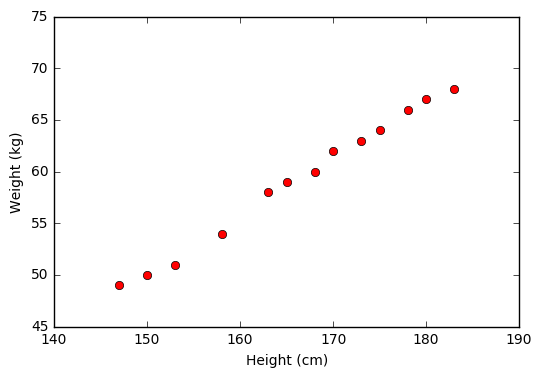
\includegraphics[width=.5\textwidth]{Chapters/03_SimpleML/3_linearregression/output_3_0.png}
%     }
% \end{figure}

Các điểm dữ liệu được minh hoạ bởi các điểm hình tròn trong Hình~\ref{fig:3_2}.
Ta thấy rằng dữ liệu được sắp xếp gần như theo một đường thẳng, vậy mô hình hồi
quy tuyến tính sau đây có khả năng cho kết quả tốt, với \pythoninline{w_0} là
hệ số điều chỉnh $b$:
\begin{center}
(cân nặng) = \pythoninline{w_1}*(chiều cao) + \pythoninline{w_0}
\end{center}


\subsection{Nghiệm theo công thức}

Tiếp theo, ta tìm các hệ số \pythoninline{w_1} và
\pythoninline{w_0} dựa vào công thức~\eqref{eqn:3_finalsolution}. Giả
nghịch đảo của một ma trận \pythoninline{A} trong Python được tính bằng
\pythoninline{numpy.linalg.pinv(A)}.% , \pythoninline{pinv} là từ viết tắt của
% \textit{pseudo inverse}.

% \begin{lstlisting}[language=Python]
% # Building Xbar 
% one = np.ones((1, X.shape[1]))
% Xbar = np.concatenate((one, X), axis = 0)

% # Calculating weights of the fitting line 
% A = np.dot(Xbar, Xbar.T)
% b = np.dot(Xbar, y)
% w = np.dot(np.linalg.pinv(A), b)
% # Preparing the fitting line 
% w_0 = w[0][0]
% w_1 = w[1][0]
% x0 = np.linspace(145, 185, 2, endpoint=True)
% y0 = w_0 + w_1*x0

% # Drawing the fitting line 
% plt.plot(X, y.T, 'ro')     # data 
% plt.plot(x0, y0)           # the fitting line
% plt.axis([140, 190, 45, 75]) # xmin, xmax, ymin, ymax 
% plt.xlabel('Height (cm)')
% plt.ylabel('Weight (kg)')
% plt.show()
% \end{lstlisting}

\begin{lstlisting}[language=Python]
# Building Xbar 
one = np.ones((X.shape[0], 1))
Xbar = np.concatenate((one, X), axis = 1) # each row is one data point 
# Calculating weights of the linear regression model
A = np.dot(Xbar.T, Xbar)
b = np.dot(Xbar.T, y)
w = np.dot(np.linalg.pinv(A), b)
# weights
w_0, w_1 = w[0], w[1]
\end{lstlisting}

% Kết quả hiển thị:
% \begin{lstlisting}[language=Python]
% w =  [[-33.73541021]
%  [  0.55920496]]
% \end{lstlisting}


% <div class="imgcap">
% <img src ="/assets/LR/output_5_1.png" align = "center">
% </div>

\begin{figure}[t]
    % caption on side
    \floatbox[{\capbeside\thisfloatsetup{capbesideposition={right,top},capbesidewidth=5.5cm}}]{figure}[\FBwidth]
    {\caption{
    Minh hoạ dữ liệu và đường thẳng xấp xỉ tìm được bởi hồi quy tuyến tính
    }
    \label{fig:3_2}}
    { % figure here
    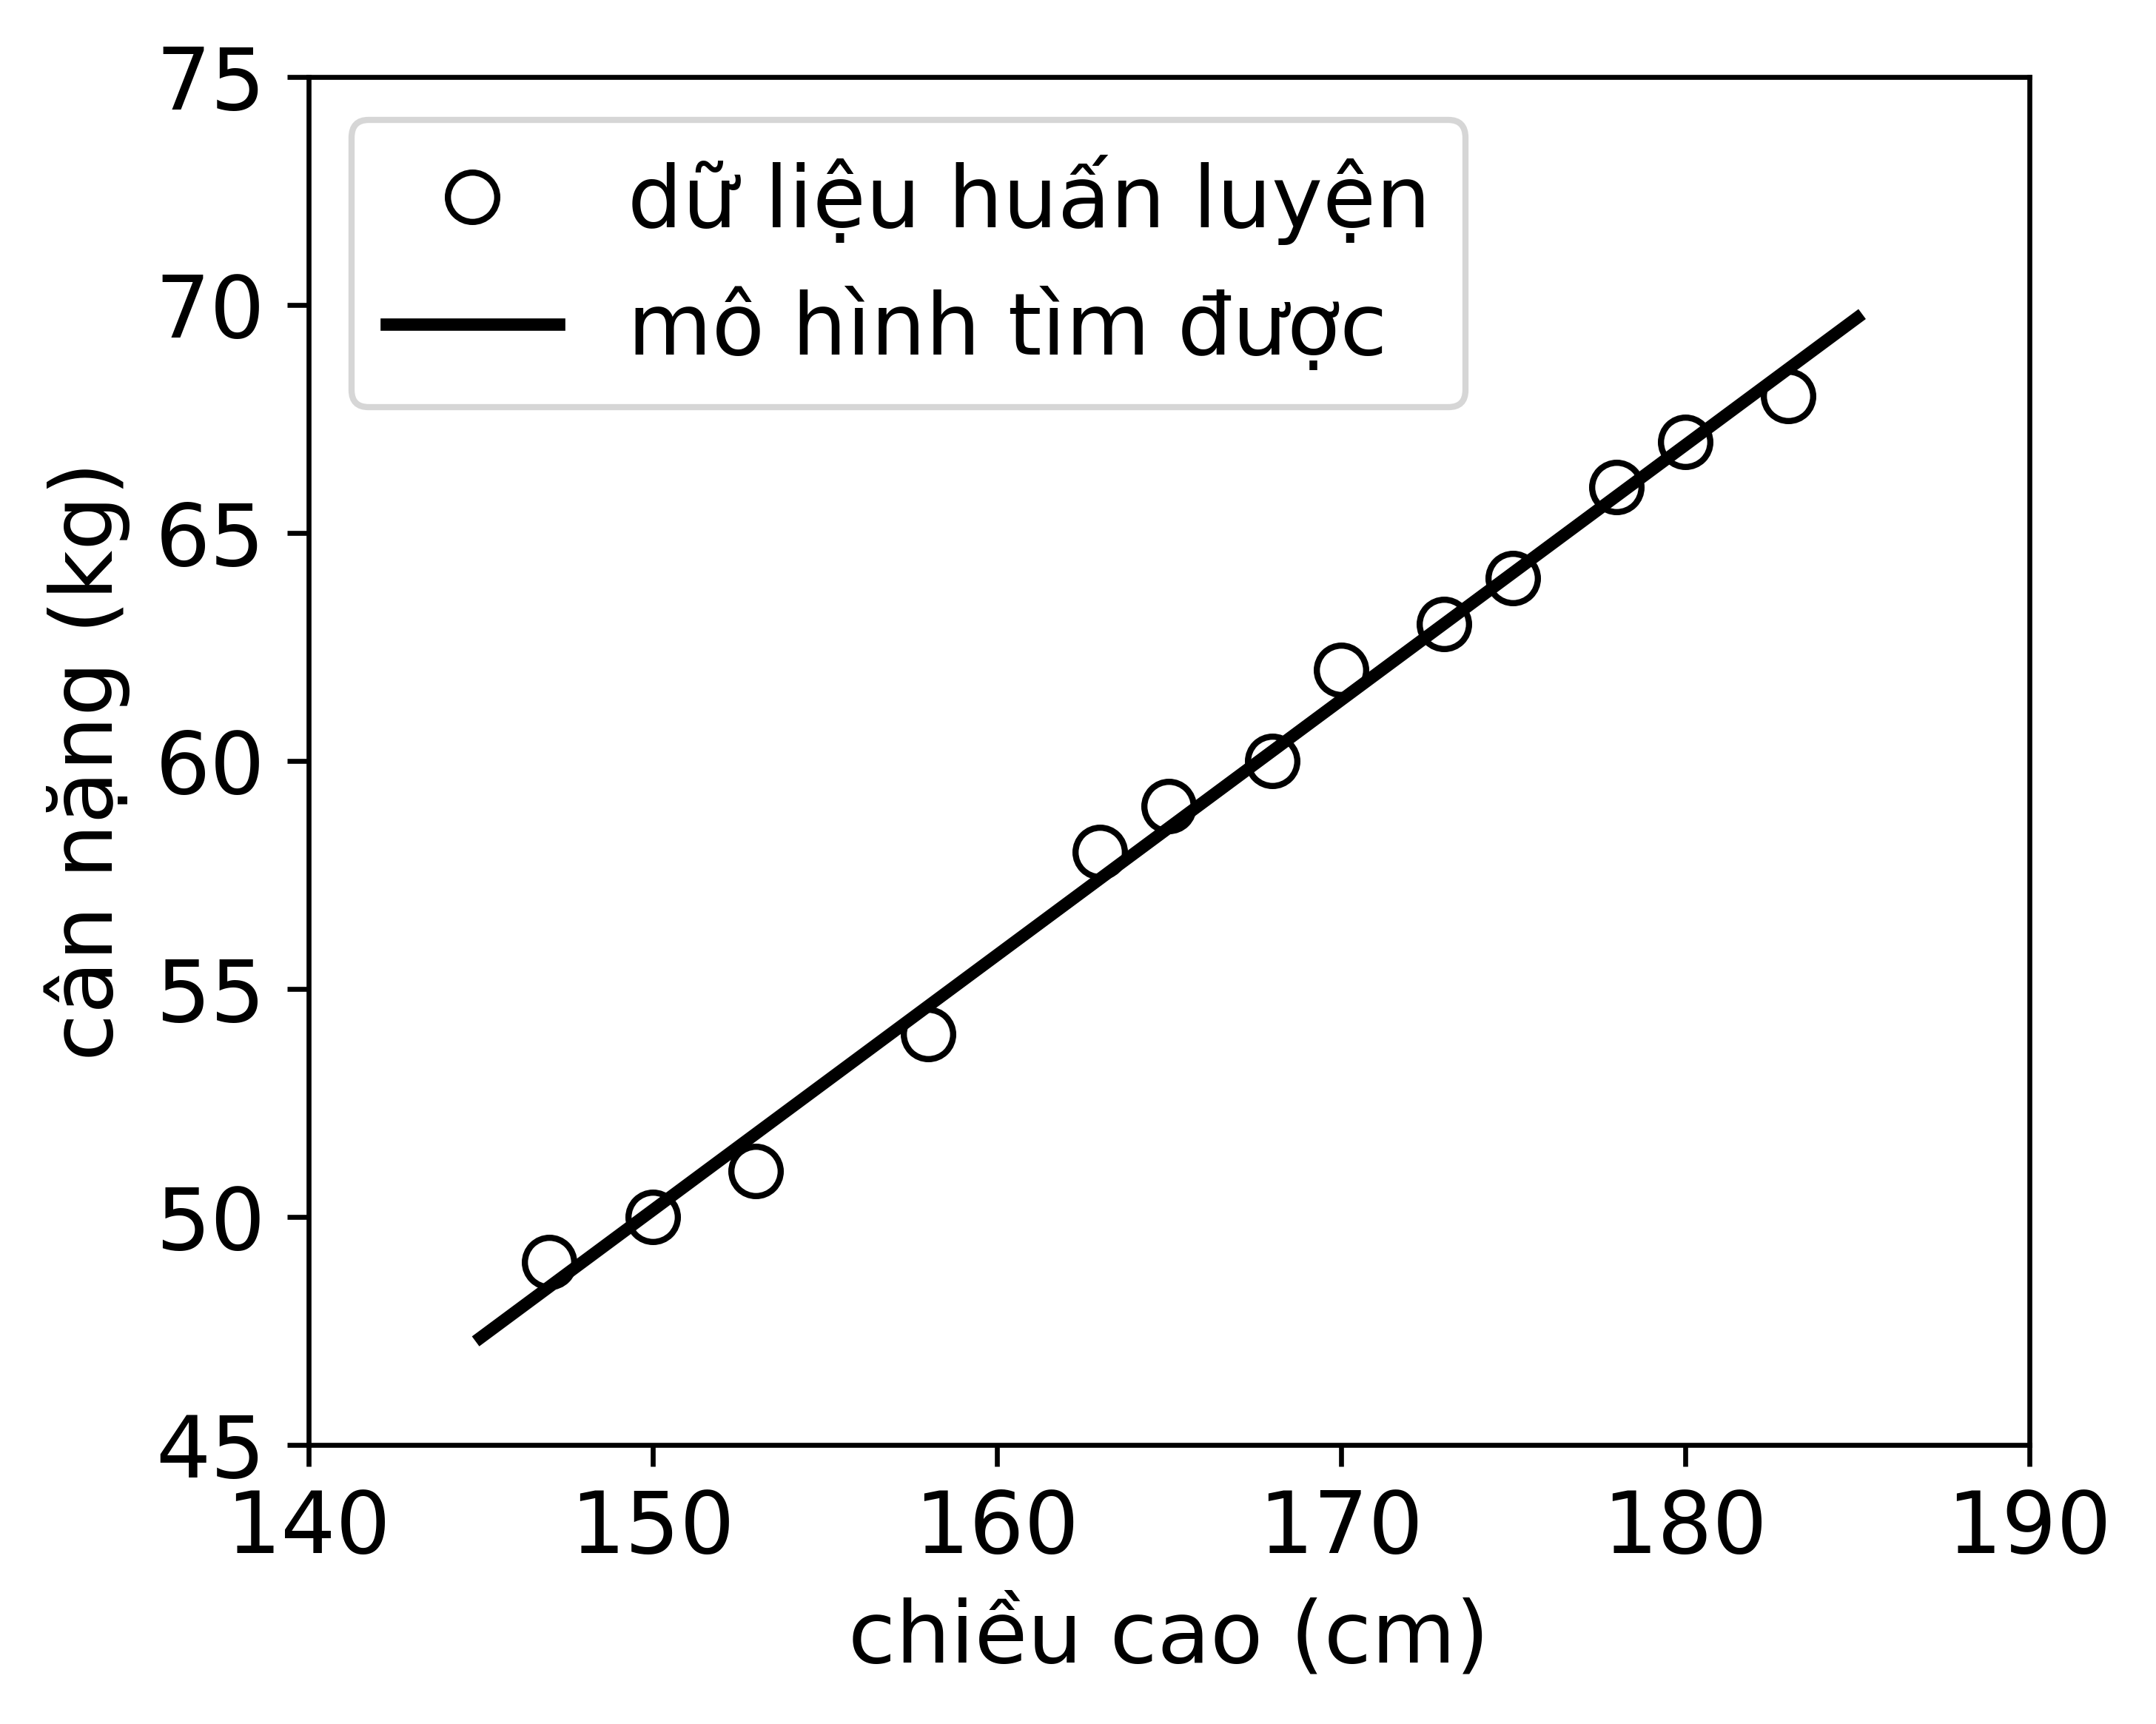
\includegraphics[width=.5\textwidth]{Chapters/03_SimpleML/3_linearregression/lr_ex.png}
    }
\end{figure}
Đường thẳng mô tả mối quan hệ giữa đầu vào và đầu ra được minh hoạ trong
Hình~\ref{fig:3_2}. Ta thấy rằng các điểm dữ liệu nằm khá gần đường thẳng dự
đoán. Vậy mô hình hồi quy tuyến tính hoạt động tốt với tập dữ liệu huấn luyện.
Bây giờ, chúng ta sử dụng mô hình này để dự đoán dữ liệu trong tập kiểm định.

\begin{lstlisting}[language=Python]
y1 = w_1*155 + w_0
y2 = w_1*160 + w_0
print('Input 155cm, true output 52kg, predicted output %.2fkg.'  %(y1) )
print('Input 160cm, true output 56kg, predicted output %.2fkg.'  %(y2) )
\end{lstlisting}
Kết quả:
\begin{lstlisting}
Input 155cm, true output 52kg, predicted output 52.94kg.
Input 160cm, true output 56kg, predicted output 55.74kg.
\end{lstlisting}

Chúng ta thấy rằng đầu ra dự đoán khá gần đầu ra thực sự.


\subsection{Nghiệm theo thư viện scikit-learn}

Tiếp theo, chúng ta sẽ sử dụng thư viện scikit-learn để tìm nghiệm.

\begin{lstlisting}[language=Python]
from sklearn import datasets, linear_model
# fit the model by Linear Regression
regr = linear_model.LinearRegression() 
regr.fit(X, y) # in scikit-learn, each sample is one row 
# Compare two results
print("scikit-learn's solution  : w_1 = ", regr.coef_[0], "w_0 = ",\        
                regr.intercept_)
print("our solution             : w_1 = ", w[1], "w_0 = ", w[0])
\end{lstlisting}
% \newpage 
Kết quả: 
\begin{lstlisting}[language=Python]
scikit-learn solution  : w_1 =  [ 0.55920496] w_0 =  [-33.73541021]
our solution           : w_1 =  [ 0.55920496] w_0 =  [-33.73541021]
\end{lstlisting}

Chúng ta thấy rằng hai kết quả thu được là như nhau.


\section{Thảo luận}


\subsection{Các bài toán có thể giải bằng hồi quy tuyến tính}
\index{hồi quy đa thức -- polynomial regression}
Hàm số $y \approx f(\bx)= \bx^T\bw + b$ là một hàm tuyến tính
theo cả $ \bw$ và $\bx$. Hồi quy tuyến tính có thể áp
dụng cho các mô hình chỉ cần tuyến tính theo $\bw$. Ví dụ
\begin{equation}
y \approx w_1 x_1 + w_2 x_2 + w_3 x_1^2 +w_4 \sin(x_2) + w_5 x_1x_2 + w_0
\end{equation}
là một hàm tuyến tính theo $\bw$ nhưng không tuyến tính theo $\bx$ nhưng vẫn có thể được giải bằng
hồi quy tuyến tính. Với mỗi vector đặc trưng $\bx=[x_1, x_2]^T $, ta
tính vector đặc trưng mới $\tilde{\bx} = [x_1, x_2, x_1^2,
\sin(x_2), x_1x_2]^T$ rồi áp dụng hồi quy tuyến tính với dữ liệu mới này. Tuy
nhiên, việc tìm ra các hàm số $\sin(x_2)$ hay $x_1x_2$ là tương đối
{không tự nhiên}. \textit{Hồi quy đa thức} (polynomial regression) thường được sử dụng nhiều hơn với các vector đặc trưng mới có dạng
$[1, x_1, x_1^2, \dots]^T$. Một ví dụ về hồi quy đa thức bậc 3 được thể hiện
trong Hình~\ref{fig:3_lra}.

% \begin{figure}[t]
%     % caption on side     
%     \floatbox[{\capbeside\thisfloatsetup{capbesideposition={right,top},capbesidewidth=6cm}}]{figure}[\FBwidth]
%     {\caption{ 
%     Polynomial regression bậc ba. 
%     }
%     \label{fig:3_polyreg}}
%     { % figure here
%     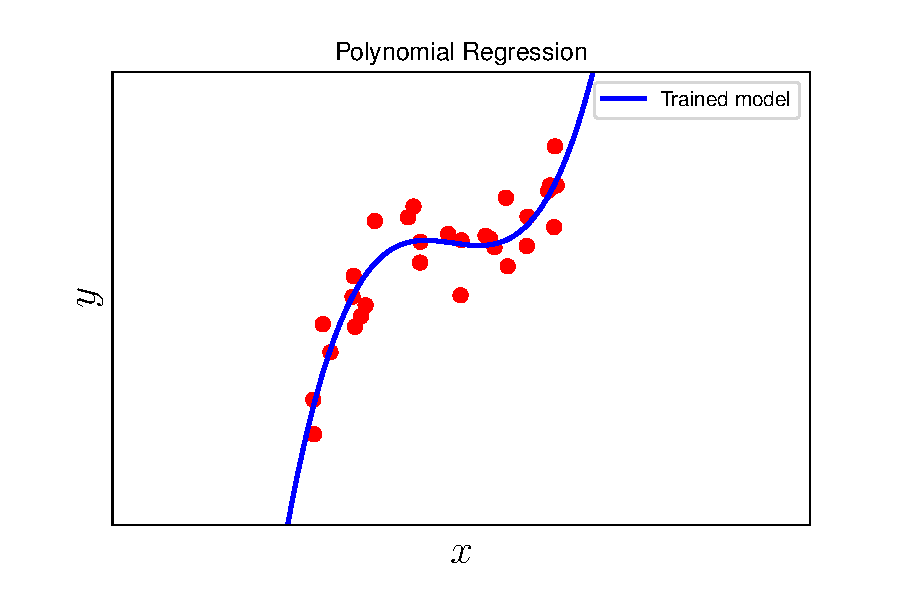
\includegraphics[width=.55\textwidth]{ebookML_src/src/linear_regression/polyregression.pdf}
%     }
% \end{figure}

%% *****************************************************************************
\begin{figure}[t]
    \begin{subfigure}{0.49\textwidth}
    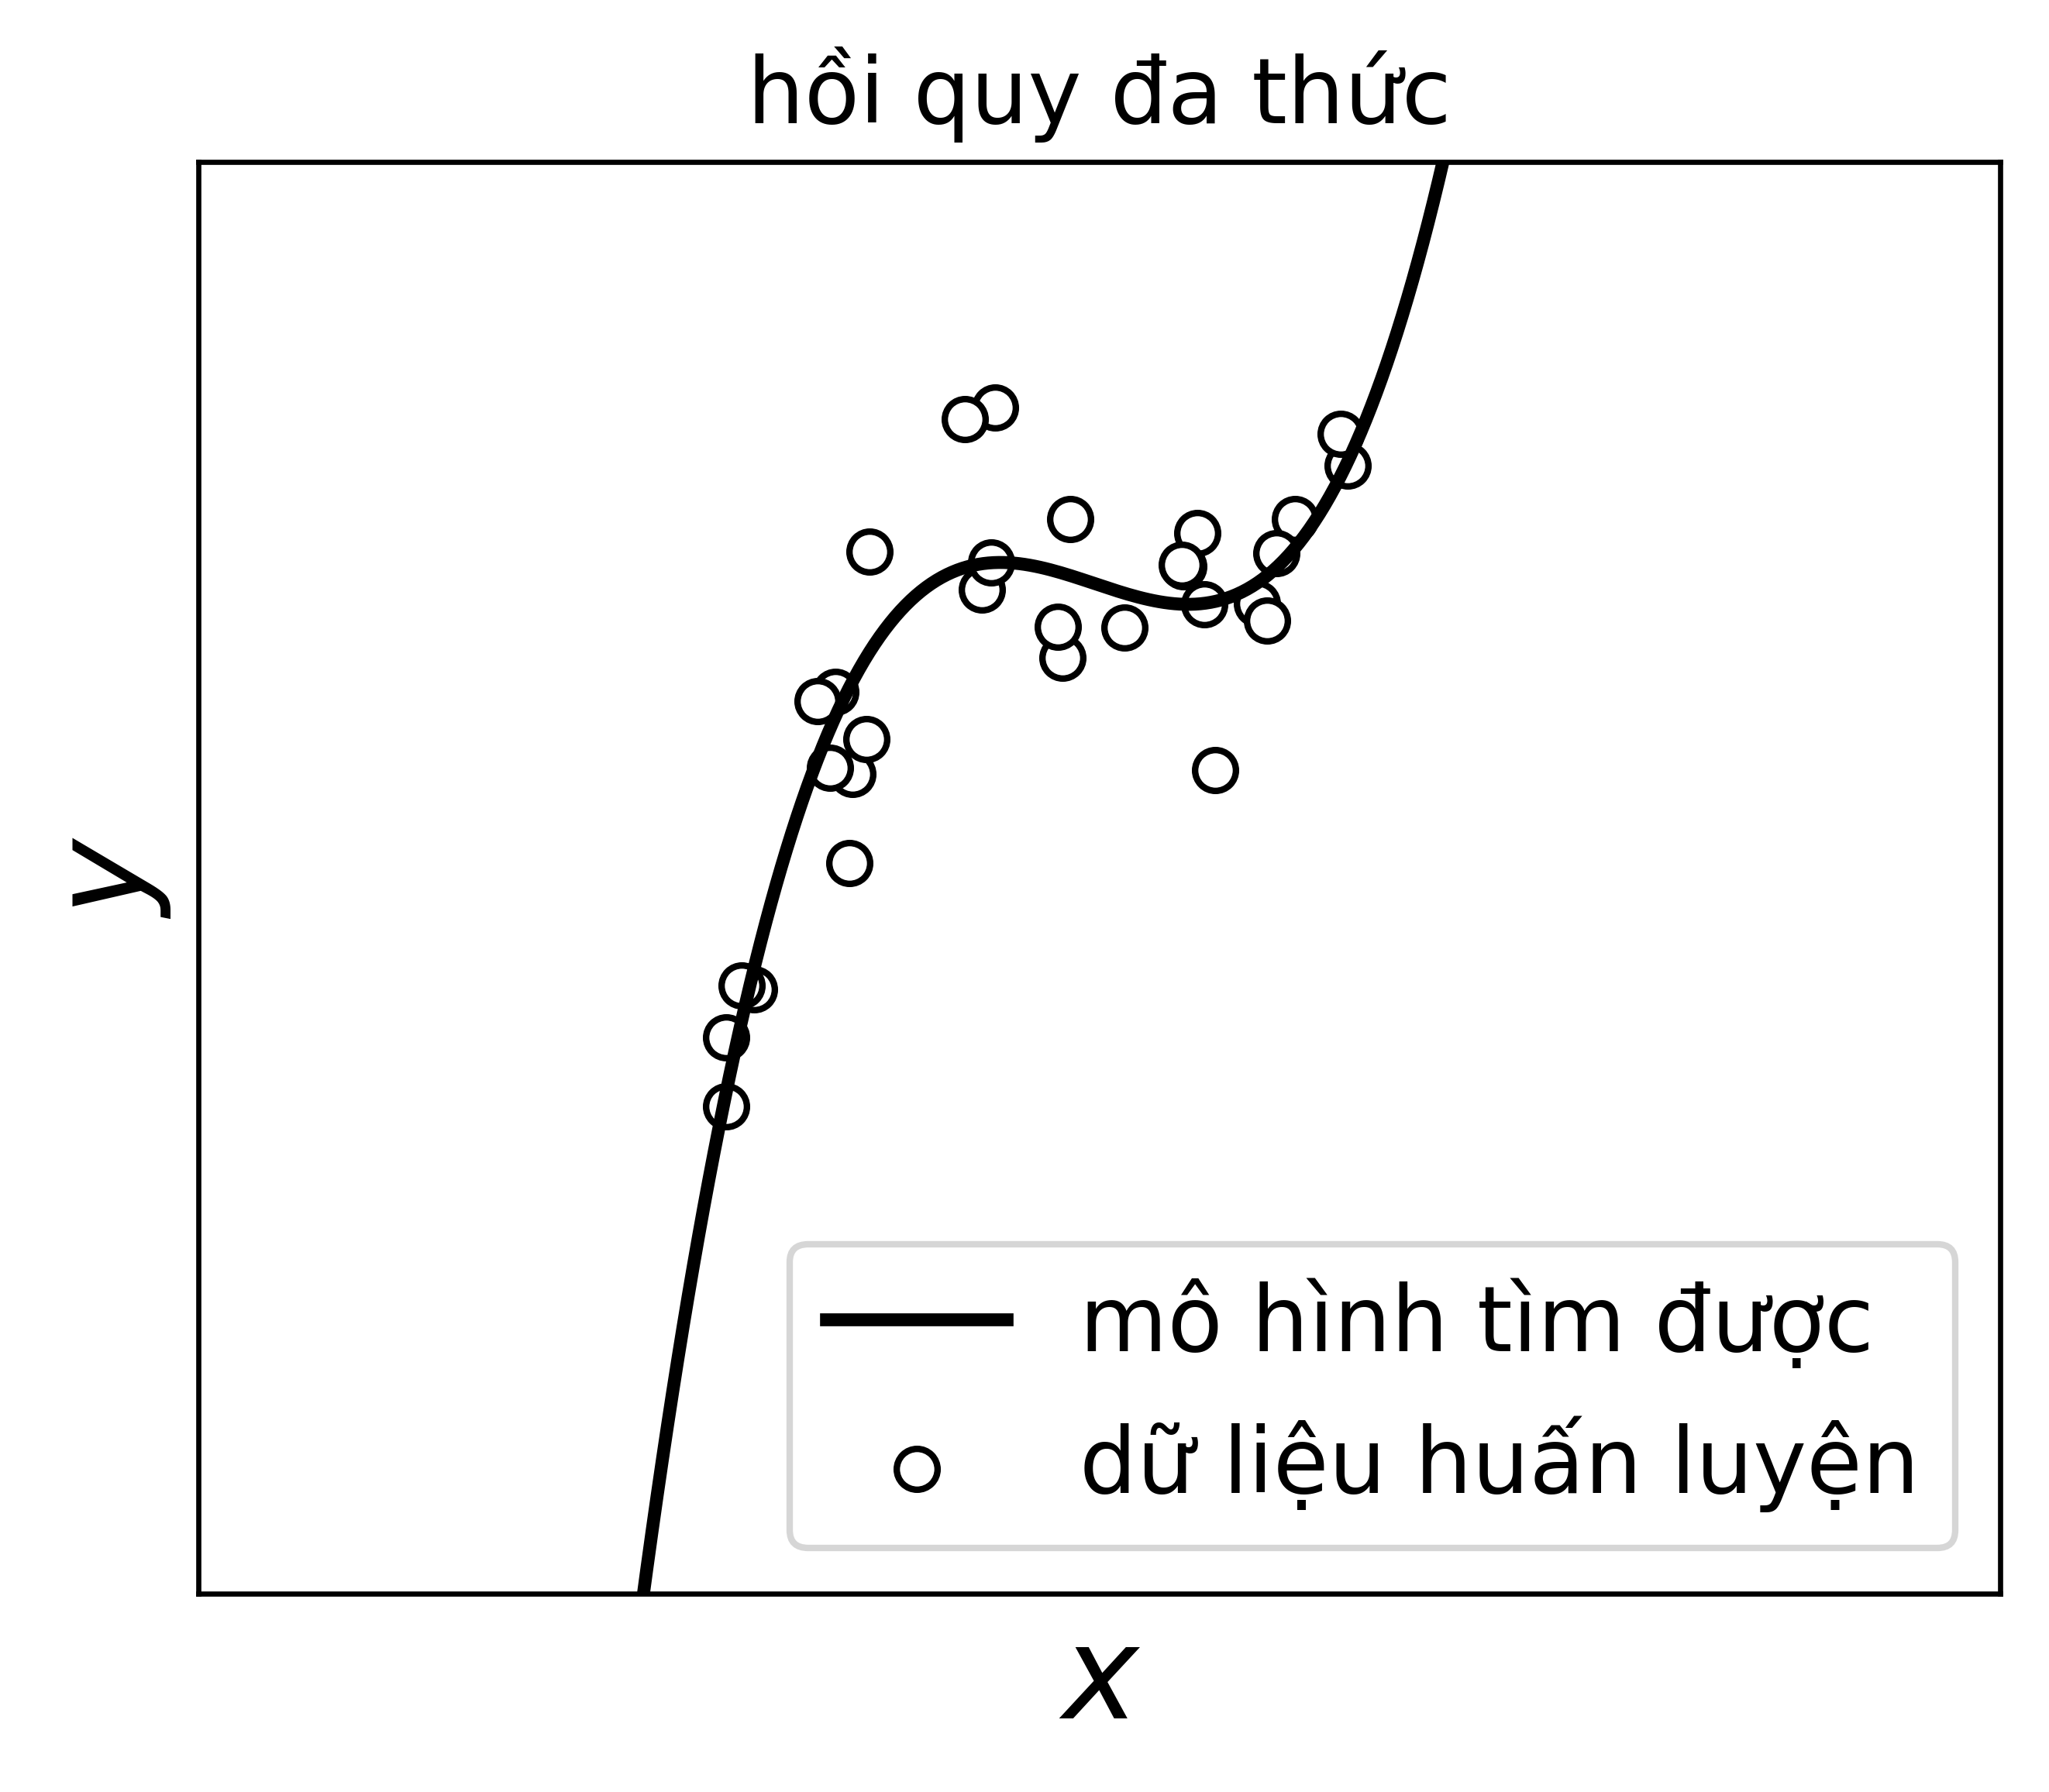
\includegraphics[width=0.99\linewidth]{Chapters/03_SimpleML/3_linearregression/polyreg.png}
    \caption{}
    \label{fig:3_lra}
    \end{subfigure}
    \begin{subfigure}{0.49\textwidth}
    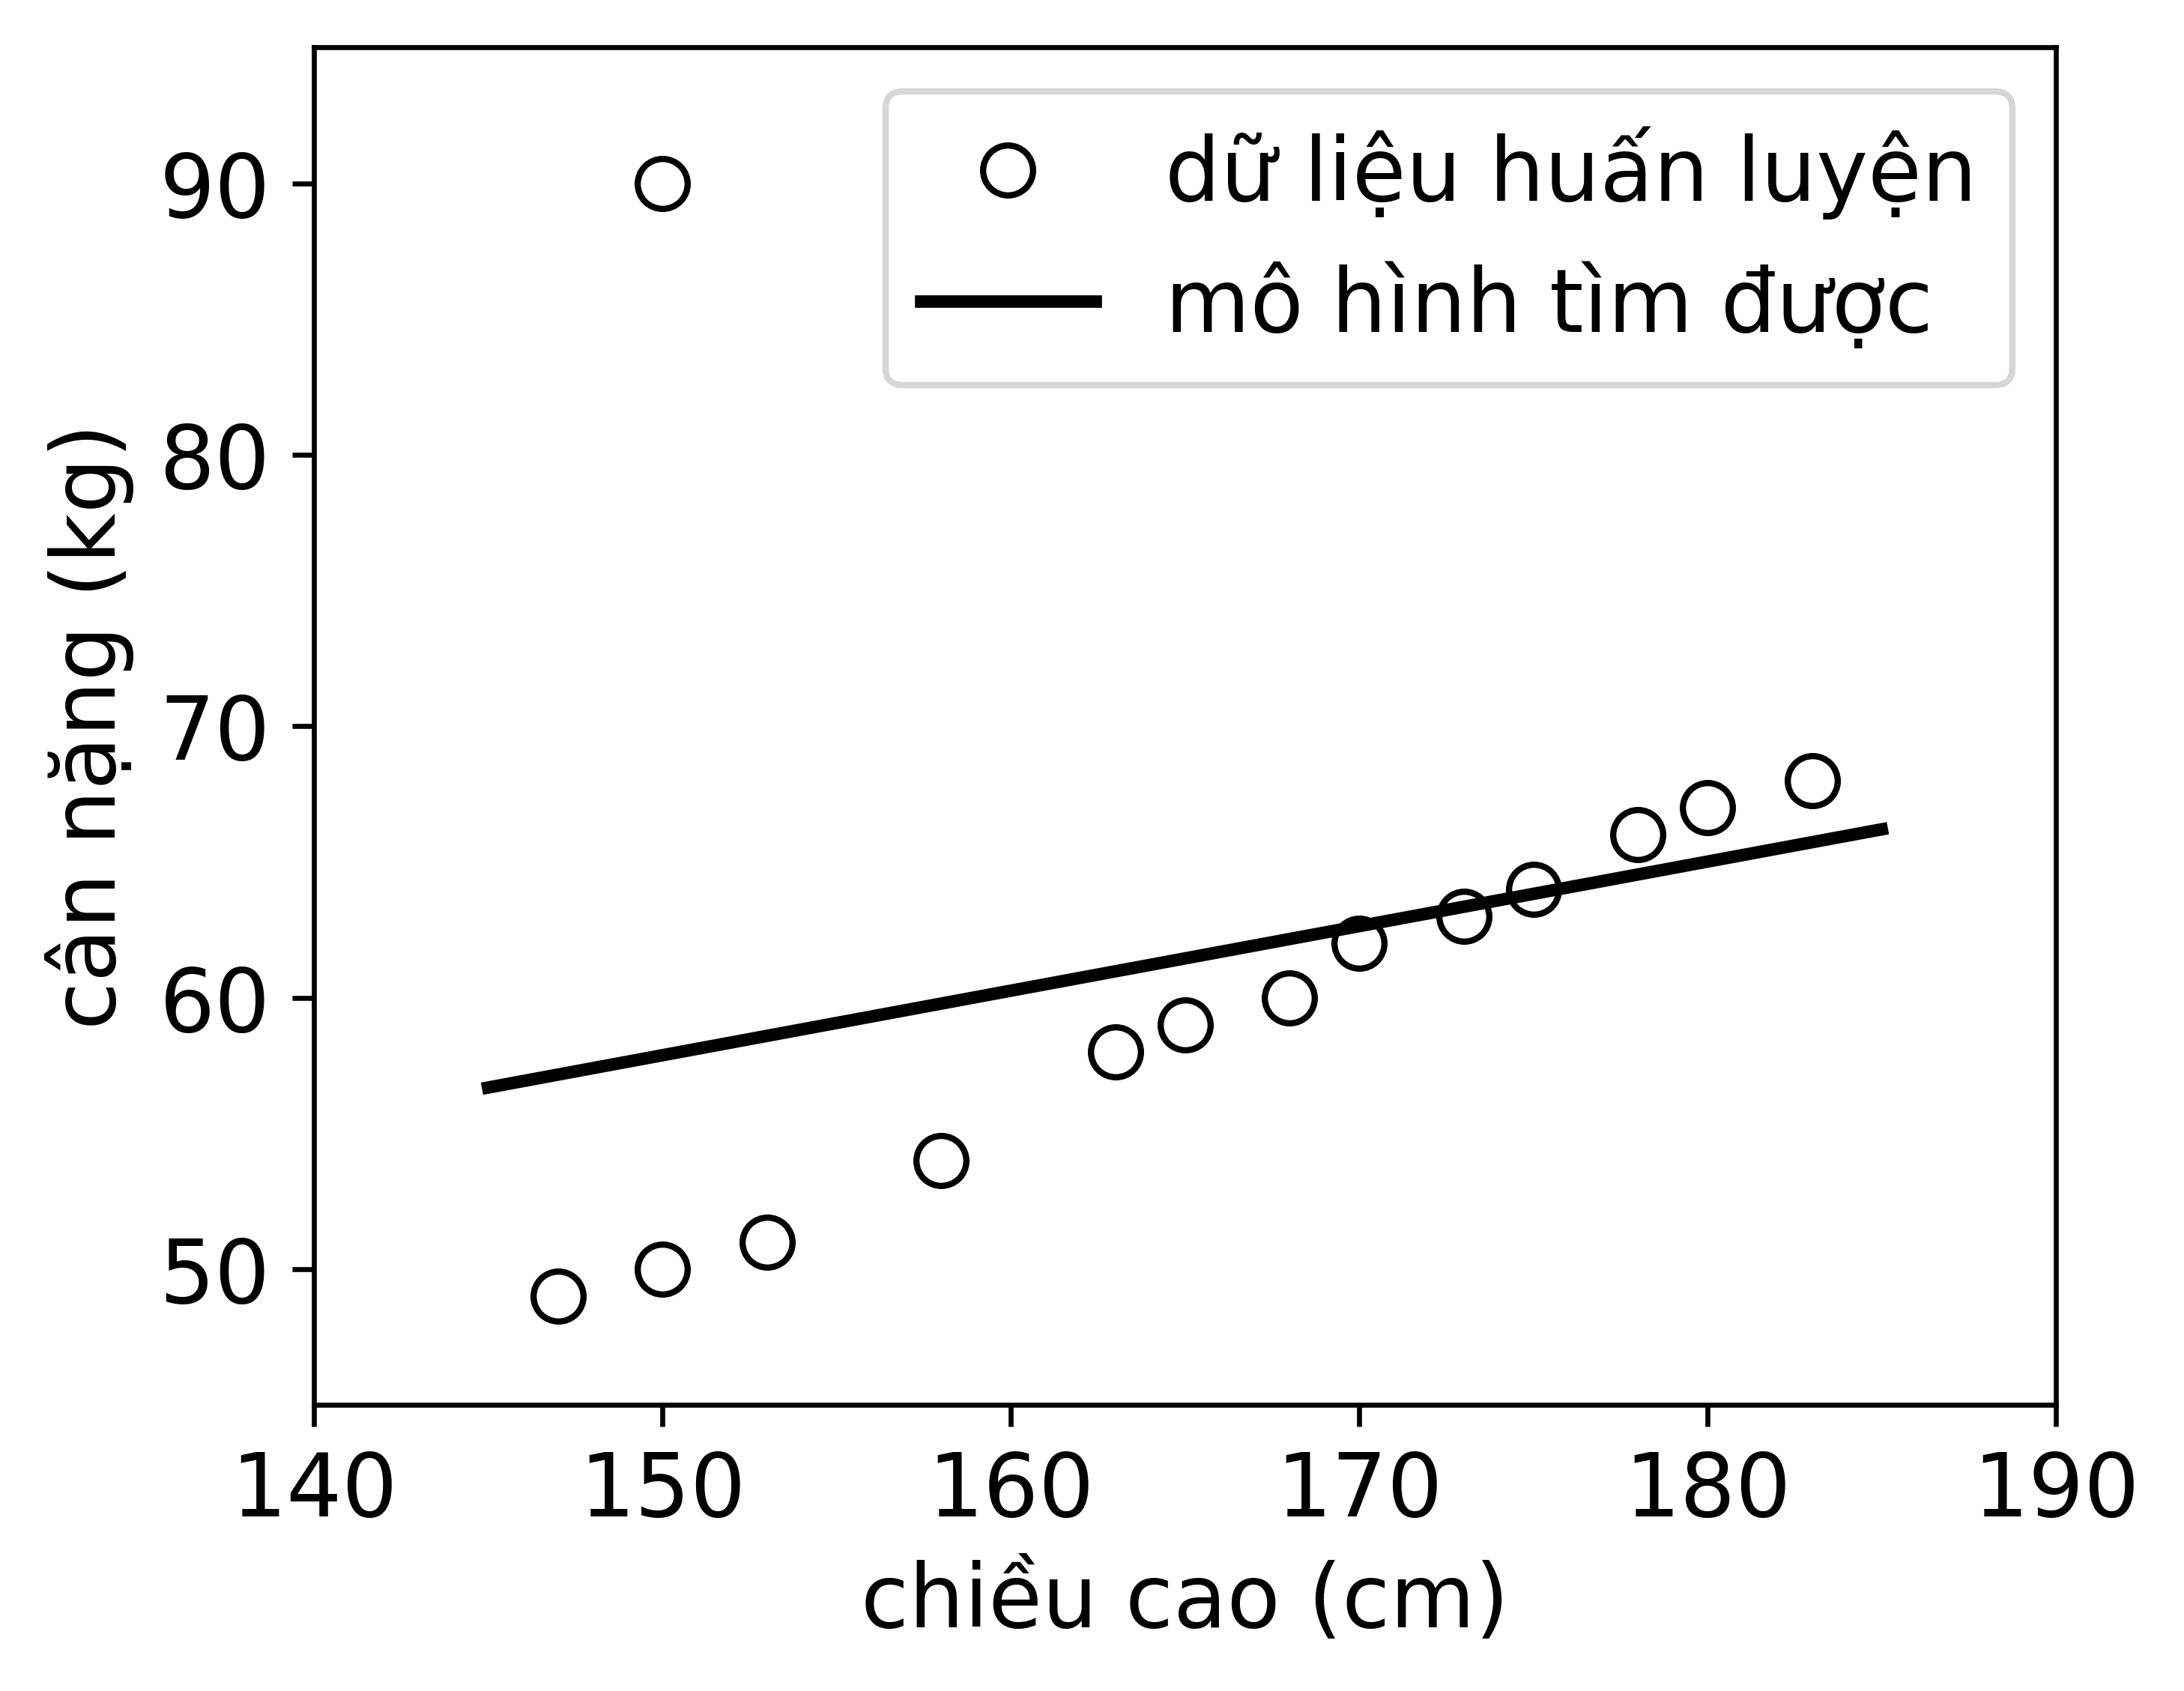
\includegraphics[width=0.99\linewidth]{ebookML_src/src/linear_regression/noise.png}
    \caption{}
    \label{fig:3_lrb}
    \end{subfigure}
    \caption{ (a) Hồi quy đa thức bậc ba (b) Hồi quy tuyến tính nhạy cảm với nhiễu. 
    }
    \label{fig:3_lr}
\end{figure}
%% *****************************************************************************



\subsection{Hạn chế của hồi quy tuyến tính}

Hạn chế đầu tiên của hồi quy tuyến tính là nó rất \textit{nhạy cảm với nhiễu} (sensitive to noise). Trong ví dụ về mối quan hệ giữa chiều cao và cân
nặng bên trên, nếu có chỉ một cặp dữ liệu {nhiễu} (150 cm, 90kg) thì kết
quả sẽ sai khác đi rất nhiều (xem Hình~\ref{fig:3_lrb}).
% \begin{figure}[t]
%     % caption on side
%     \floatbox[{\capbeside\thisfloatsetup{capbesideposition={right,top},capbesidewidth=6cm}}]{figure}[\FBwidth]
%     {\caption{
%     Linear regression hoạt động không tốt khi có nhiễu.
%     }
%     \label{fig:3_withnoise}}
%     { % figure here
%     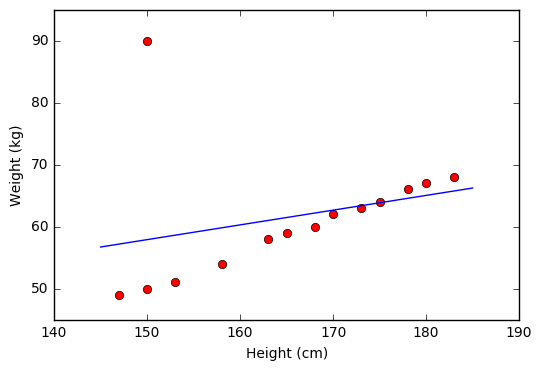
\includegraphics[width=.5\textwidth]{Chapters/03_SimpleML/3_linearregression/output_13_1.png}
%     }
% \end{figure}

\index{hồi quy Huber -- Huber regression}

Một kỹ thuật giúp tránh hiện tượng này là loại bỏ các nhiễu trong quá trình tìm nghiệm. Việc làm này có thể phức tạp và tương đối tốn thời gian. Có một cách khác giúp tránh công việc loại bỏ nhiễu là sử dụng \textit{mất mát Huber}\footnote{\url{https://goo.gl/TBUWzg}}. Hồi quy tuyến tính với mất mát Huber được gọi là \textit{hồi quy Huber}, được khẳng định là có khả năng kháng nhiễu tốt hơn. Xem thêm \textit{Huber Regressor, scikit learn} (\url{https://goo.gl/h2rKu5}).

Hạn chế thứ hai của hồi quy tuyến tính là nó \textit{không biễu diễn được các mô
hình phức tạp}. Mặc dù ta thấy rằng phương pháp này có thể được áp dụng nếu quan
hệ giữa đầu ra và đầu vào là phi tuyến, nhưng mối quan hệ này vẫn đơn giản hơn
nhiều so với các mô hình thực tế. Hơn nữa, việc tìm ra các đặc trưng $x_1^2,
\sin(x_2), x_1x_2$ như trên là không khả thi khi số chiều dữ liệu lớn lên.


\subsection{Hồi quy ridge}
\index{hồi quy ridge -- ridge regression}

Có một kỹ thuật nhỏ giúp tránh trường hợp $\bX\bX^T$ không khả nghịch là biến nó thành $\bA = \bX\bX^T + \lambda\bI$ với $\lambda$ là một số dương nhỏ
và $\bI$ là ma trận đơn vị với bậc phù hợp. 

Ma trận $\bA$ là khả nghịch vì nó là một ma trận xác định dương. Thật vậy, với
mọi $\bw \neq \bzero$,
\begin{equation*}
    \bw^T\bA\bw = \bw^T(\bX\bX^T + \lambda \bI) \bw = \bw^T\bX\bX^T\bw  +
    \lambda \bw^T\bw = \|\bX^T\bw\|_2^2 + \lambda \|\bw\|_2^2 > 0.
\end{equation*}
Lúc này, nghiệm của bài toán là $\by = (\bX \bX^T + \lambda \bI)^{-1} \bX\by$.

Xét hàm mất mát
\begin{equation}
    \label{eqn:3_ridge}
    \L_2(\bw) = \frac{1}{2N}(\|\by - \bX^T\bw\|_2^2 + \lambda\|\bw\|_2^2).
\end{equation}
Phương trình gradient theo $\bw$ bằng không: 
\begin{equation}
    \frac{\nabla \L_2(\bw)}{\nabla \bw} = \bzero \Leftrightarrow
    \frac{1}{N}(\bX(\bX^T\bw - \by) + \lambda \bw) = \bzero \Leftrightarrow
    (\bX\bX^T + \lambda \bI) \bw = \bX\by 
\end{equation}
Ta thấy $\bw = (\bX\bX^T + \lambda\bI)^{-1}\bX\by$ chính là nghiệm của
bài toán tối thiểu $\L_2(\bw)$ trong~\eqref{eqn:3_ridge}. Mô hình machine learning với hàm mất mát~\eqref{eqn:3_ridge} còn được
gọi là \textit{hồi quy ridge}. 
 Ngoài việc giúp phương trình gradient theo hệ số bằng không có nghiệm duy
nhất, hồi quy ridge còn giúp mô hình tránh được overfitting như sẽ thấy trong Chương~\ref{cha:overfitting}. 

\subsection{Phương pháp tối ưu khác}


Hồi quy tuyến tính là một mô hình đơn giản, lời giải cho phương trình gradient
bằng không cũng không phức tạp. {Trong hầu hết các trường hợp, việc giải các
phương trình gradient bằng không tương đối phức tạp.} Tuy nhiên, nếu ta tính được đàm hàm của hàm mất mát, các tham số mô hình có thể được giải bằng một phương pháp hữu dụng có tên \textit{gradient descent}. Trên thực tế, một vector đặc trưng có thể
có kích thước rất lớn, dẫn đến ma trận $\bX\bX^T$ cũng có kích thước lớn và việc
tính ma trận nghịch đảo có thể không lợi về mặt tính toán. Gradient descent sẽ
giúp tránh được việc tính ma trận nghịch đảo. Chúng ta sẽ hiểu kỹ hơn về phương
pháp này trong Chương~\ref{cha:gradient_descent}.

% \subsection{Đọc thêm}
% \begin{enumerate}
%     \item \textit{Simple Linear Regression Tutorial for Machine Learning} (\url{https://goo.gl/WRVda8}).

%     \item \textit{Regularization: Ridge Regression and the LASSO} (\url{https://goo.gl/uRzN1K}).
% \end{enumerate}
 